\chapter{Introducción Específica} % Main chapter title
\label{Chapter2}

\definecolor{mygreen}{rgb}{0,0.6,0}
\definecolor{mygray}{rgb}{0.5,0.5,0.5}
\definecolor{mymauve}{rgb}{0.58,0,0.82}

\lstset{ %
  backgroundcolor=\color{white},   % choose the background color; you must add \usepackage{color} or \usepackage{xcolor}
  basicstyle=\large,        % the size of the fonts that are used for the code
  breakatwhitespace=false,         % sets if automatic breaks should only happen at whitespace
  breaklines=true,                 % sets automatic line breaking
  captionpos=b,                    % sets the caption-position to bottom
  commentstyle=\color{mygreen},    % comment style
  deletekeywords={...},            % if you want to delete keywords from the given language
  %escapeinside={\%*}{*)},          % if you want to add LaTeX within your code
  %extendedchars=true,              % lets you use non-ASCII characters; for 8-bits encodings only, does not work with UTF-8
  %frame=single,	                   % adds a frame around the code
  keepspaces=true,                 % keeps spaces in text, useful for keeping indentation of code (possibly needs columns=flexible)
  keywordstyle=\color{blue},       % keyword style
  language=[ANSI]C,					% the language of the code
  %otherkeywords={*,...},           % if you want to add more keywords to the set
  numbers=none,                    % where to put the line-numbers; possible values are (none, left, right)
  numbersep=5pt,                   % how far the line-numbers are from the code
  numberstyle=\tiny\color{mygray}, % the style that is used for the line-numbers
  rulecolor=\color{black},         % if not set, the frame-color may be changed on line-breaks within not-black text (e.g. comments (green here))
  showspaces=false,                % show spaces everywhere adding particular underscores; it overrides 'showstringspaces'
  showstringspaces=false,          % underline spaces within strings only
  showtabs=false,                  % show tabs within strings adding particular underscores
  stepnumber=1,                    % the step between two line-numbers. If it's 1, each line will be numbered
  stringstyle=\color{mymauve},     % string literal style
  tabsize=2,	                   % sets default tabsize to 2 spaces
  title=\lstname,                   % show the filename of files included with \lstinputlisting; also try caption instead of title
  morecomment=[s]{/*}{*/}%
}



En este capítulo se identifican aspectos relevante de la planificación. Asimismo, se describen las herramientas empleadas para la realización de este trabajo.

%----------------------------------------------------------------------------------------
%	SECTION 1
%----------------------------------------------------------------------------------------
\section{Requerimientos}
\label{sec:requerimientos}

A continuación se enumeran los requerimientos del proyecto:

\begin{enumerate}
  \item Requerimientos de documentación:
   \begin{enumerate}
     \item Se debe generar un Memoria Técnica con la documentación de ingeniería detallada.
	   \item Se debe generar un documento de casos de prueba.
	 \end{enumerate}
	\item Requerimientos funcionales del sistema:
	\begin{enumerate}
		\item El sistema debe adquirir datos de un array de sensores de temperatura a intervalos regulares con un período de adquisición seleccionable.
		\item El sistema debe adquirir datos de un anemómetro a intervalos regulares con un período de adquisición seleccionable.
		\item El sistema debe almacenar los datos de temperatura y velocidad de viento adquiridas junto con una marca de tiempo identificatoria en un medio físico no volátil.
		\item El sistema debe poder operar con dos perfiles de consumo de energía: máximo desempeño y mínimo consumo de energía, respectivamente.
		\item El sistema debe contar con una interfaz serie cableada que permita realizar operaciones de configuración y mantenimiento.
	\end{enumerate}
	\item Requerimientos de verificación:
	\begin{enumerate}
		\item Se debe generar una matriz de trazabilidad entre la Memoria Técnica y los requerimientos.
		\item Se debe generar una matriz de trazabilidad entre las pruebas de integración y los requerimientos.
	\end{enumerate}
	\item Requerimientos de validación:
	\begin{enumerate}
	  \item Se debe generar una matriz de trazabilidad entre el documento de casos de prueba y los requerimientos.
  \end{enumerate}
\end{enumerate}

\section{Planificación}
\label{sec:plan}

La planificación completa del proyecto puede encontrarse publicada en la web del Laboratorio de Sistemas Embebidos de FIUBA \citep{plan}.

A los fines de facilitar la comprensión del trabajo realizado, se detallan en la tabla \ref{tab:planificacion} las etapas del proyecto junto con la cantidad de horas destinadas y los hitos a alcanzar en cada una de ellas.  Puede observarse que el proyecto insume 600 horas de trabajo en total.

\vspace{20px}

% Please add the following required packages to your document preamble:
% \usepackage{multirow}
\begin{table}[ht]
\centering
\caption[Etapas principales del proyecto]{Etapas principales del proyecto. Se detallan de las horas planificadas y los hitos a alcanzar en cada etapa.}
\label{tab:planificacion}
\begin{tabular}{lcl}
\toprule
\textbf{Etapa}                            & \textbf{Horas}       & \textbf{Hitos}                                \\ \midrule
\multirow{2}{*}{Documentación y análisis} & \multirow{2}{*}{100} & Plan de trabajo                             \\
                                          &                      & Presentación de plan de trabajo \vspace{5px}\\
                                          & \multicolumn{1}{l}{} &                                             \\ 
Diseño e implementación                   & 340                  & Documentación de submódulos  \vspace{5px}   \\
                                          & \multicolumn{1}{l}{} &                                             \\ 
               							  &                      & Reporte de pruebas unitarias                \\
Verificación y validación                 & 60                   & Reporte de pruebas de integración           \\
                                          &                      & Reporte de casos de prueba   \vspace{5px}   \\
                                          & \multicolumn{1}{l}{} &                                             \\ 
\multirow{2}{*}{Proceso de cierre}        & \multirow{2}{*}{100} & Memoria Técnica                             \\
                                          &                      & Presentación de Trabajo Final               \\ \bottomrule
\end{tabular}
\end{table}

\vspace{20px}

Para cada una de las etapas del proyecto, se realizó un desglose de tareas procurando que la duración de cada una no supere las 40 horas, para mejorar el proceso de control y seguimiento.

Las tareas identificadas se arreglaron esquemáticamente en el diagrama de \textit{Activity on Node} que se ilustra en la figura \ref{fig:AoN}. Se utiliza un mismo color para identificar las distintas tareas que componen una misma etapa del proyecto según la tabla \ref{tab:planificacion}. En color amarillo se detacan las tareas de la etapa de documentación y análisis; en celeste las tareas de diseño e implementación; en verde las tareas de verificación y validación y finalmente, en color rojo, las tareas que componen el proceso de cierre. 

En el diagrama, los tiempos de duración de las tareas están representados con la variable $t$ y expresados en horas. Asimismo, las tareas poseen un código numérico único que fue usado para realizar la trazabilidad de los requerimientos en las distintas etapas del proyecto.

Cabe destacar que dentro de las tareas de planificación, se incluyó la definición de casos de prueba.  Se considera que fue una decisión acertada por el mejor entendimiento que se logró sobre las características de diseño que debía contener el sistema. Asimismo, esto permitió descartar características que se pensaban implementar pero que no respondían al cumplimiento de ningún requerimiento. 

\begin{figure}[htpb]
	\centering
	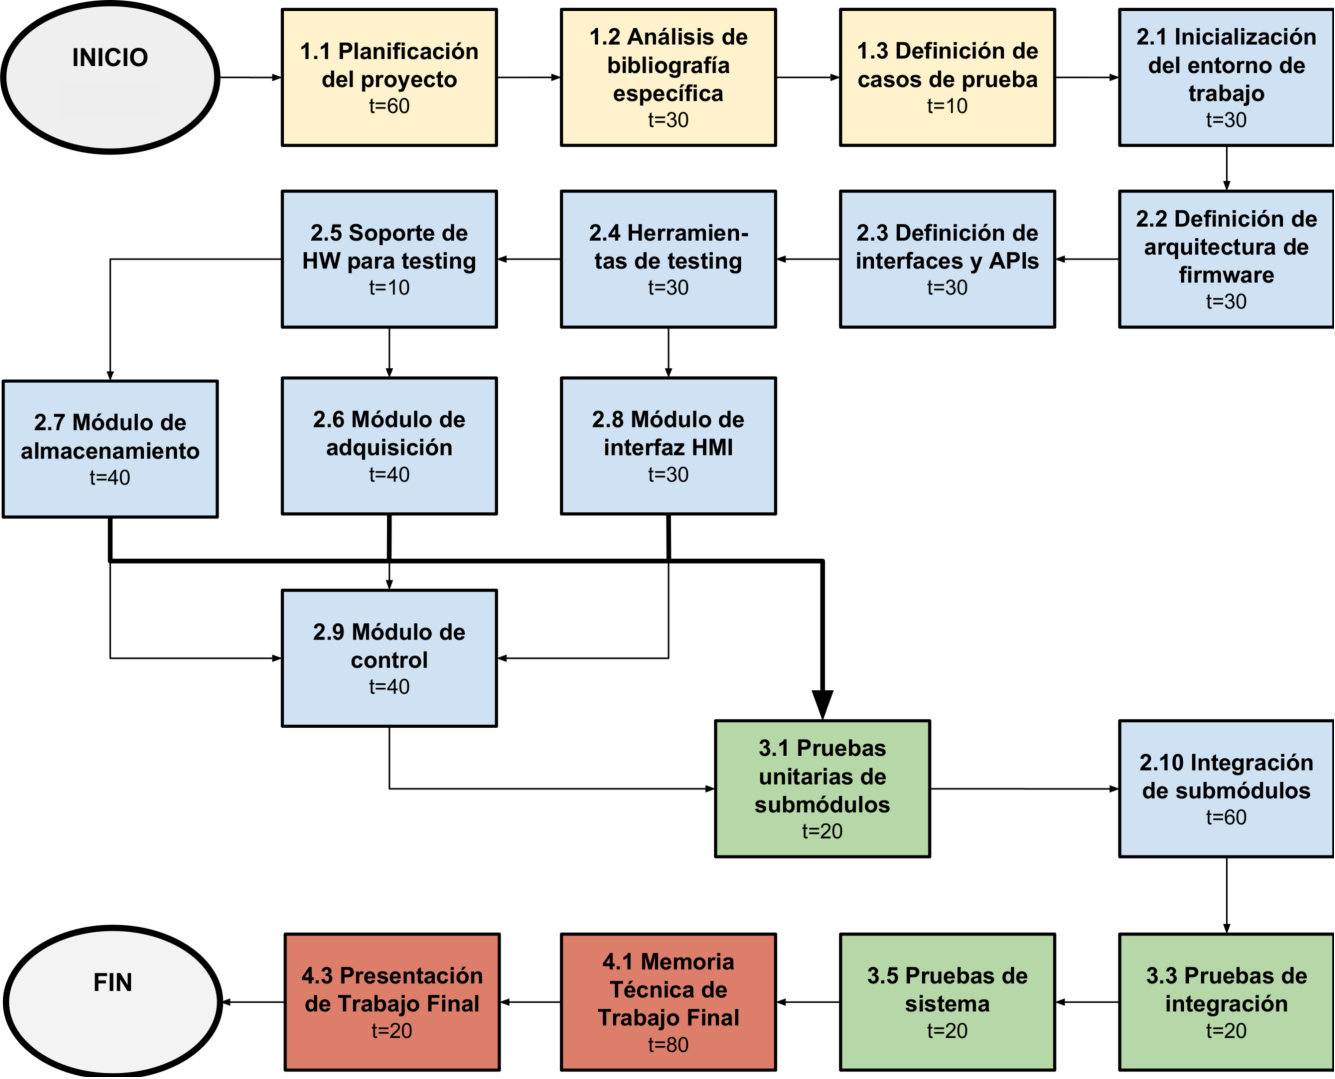
\includegraphics[width=\textwidth]{./Figures/AoN.pdf}
	\caption[Diagrama \textit{Activity on Node}.]{Diagrama \textit{Activity on Node}.  En colores puede distinguirse: en amarillo la etapa de documentación y análisis preliminar; en azul la etapa de diseño e implementación; en verde la etapa de verificación y validación y en rojo el proceso de cierre. El tiempo t está expresado en horas.}
	\label{fig:AoN}
\end{figure}

%\clearpage



\section{Metodología}

En esta sección se describen los aspectos metodológicos relevantes que se aplicaron durante el desarrollo del trabajo.  

\subsection{Control de versiones}
\label{subsec:branching}

Se adoptó un modelo de desarrollo creado por Vincent Driessen llamado ``\textit{A successful Git branching model''} \citep{Driessen}.  El modelo está basado en la herramienta de control de versiones \textit{git} y consiste en un conjunto de procedimientos para ordenar y sistematizar el flujo de trabajo. Este modelo propone utilizar un repositorio considerado a los fines prácticos ``central'' (en git todos los repositorios son idénticos) llamado \textit{origin}.  Todos los desarrolladores trabajan contra este repositorio central con las operaciones típicas de \textit{push} y \textit{pop}.  

Adicionalmente, puede haber intercambios entre los repositorios de los distintos desarrolladores que formen un mismo equipo de trabajo. Estos intercambios pueden visualizarse en la figura \ref{fig:esquema-repos}, donde se esquematizan, por un lado, los posibles flujos de trabajo entre el repositorio \textit{origin} y los distintos desarrolladores, y por el otro, entre los repositorios propios de cada desarrollador. 

\begin{figure}[ht]
	\centering
	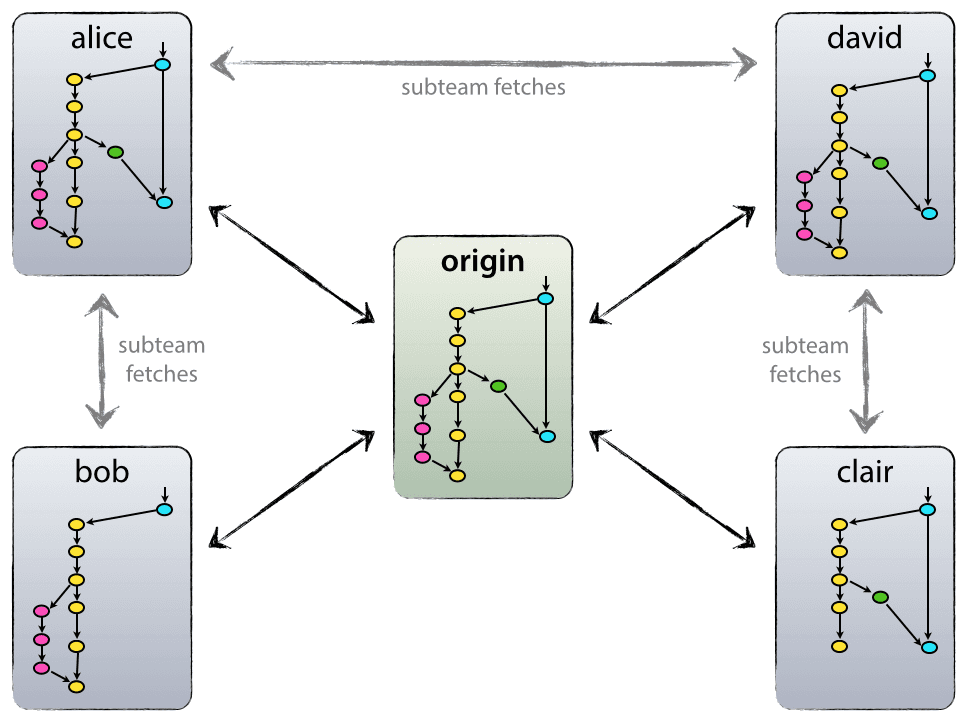
\includegraphics[width=.6\textwidth]{./Figures/centr-decentr@2x.png}
	\caption[Esquema del flujo de trabajo entre repositorios]{Esquema del flujo de trabajo entre repositorios\protect\footnotemark.}
	\label{fig:esquema-repos}
\end{figure}

\footnotetext{Imagen tomada de \url{https://nvie.com/img/centr-decentr@2x.png}.}

Para la elaboración de este trabajo, donde la codificación recayó principalmente sobre una sóla persona, no fueron habituales las operaciones contra un repositorio distinto de \textit{origin}, implementado en \textit{github}. Sin embargo, se considera la experiencia de apropiación de la metodología de trabajo muy valiosa para la formación profesional, ya que el autor de este trabajo no había tenido oportunidad de trabajar tan extensa y sistemáticamente con control de versiones previamente.

En cuanto a la estrategia de uso de ramas, siguiendo el modelo adoptado, se dispuso de dos ramas principales llamadas \textit{master} y \textit{develop}.  En \textit{origin/master} sólo se incluyen \textit{commits} con versiones estables con capacidad de ser puestas en producción, es decir sobre el prototipo de manera que éste pueda operar satisfactoriamente.  En \textit{origin/develop} se encuentran  los últimos cambios que integran las diferentes características ya logradas del código.  Cuando la rama \textit{develop} alcanza un punto de estabilidad y madurez suficiente se debe hacer un \textit{merge} con \textit{master}.% y generar un nuevo número de \textit{release}.

En términos generales, el esquema de ramas propuesto por el modelo de Vincent Driessen puede observar en la figura  \ref{fig:branching} donde se explicitan las posibles interacciones entre ramas.

\vfill

\begin{figure}[!htbp]
	\centering
	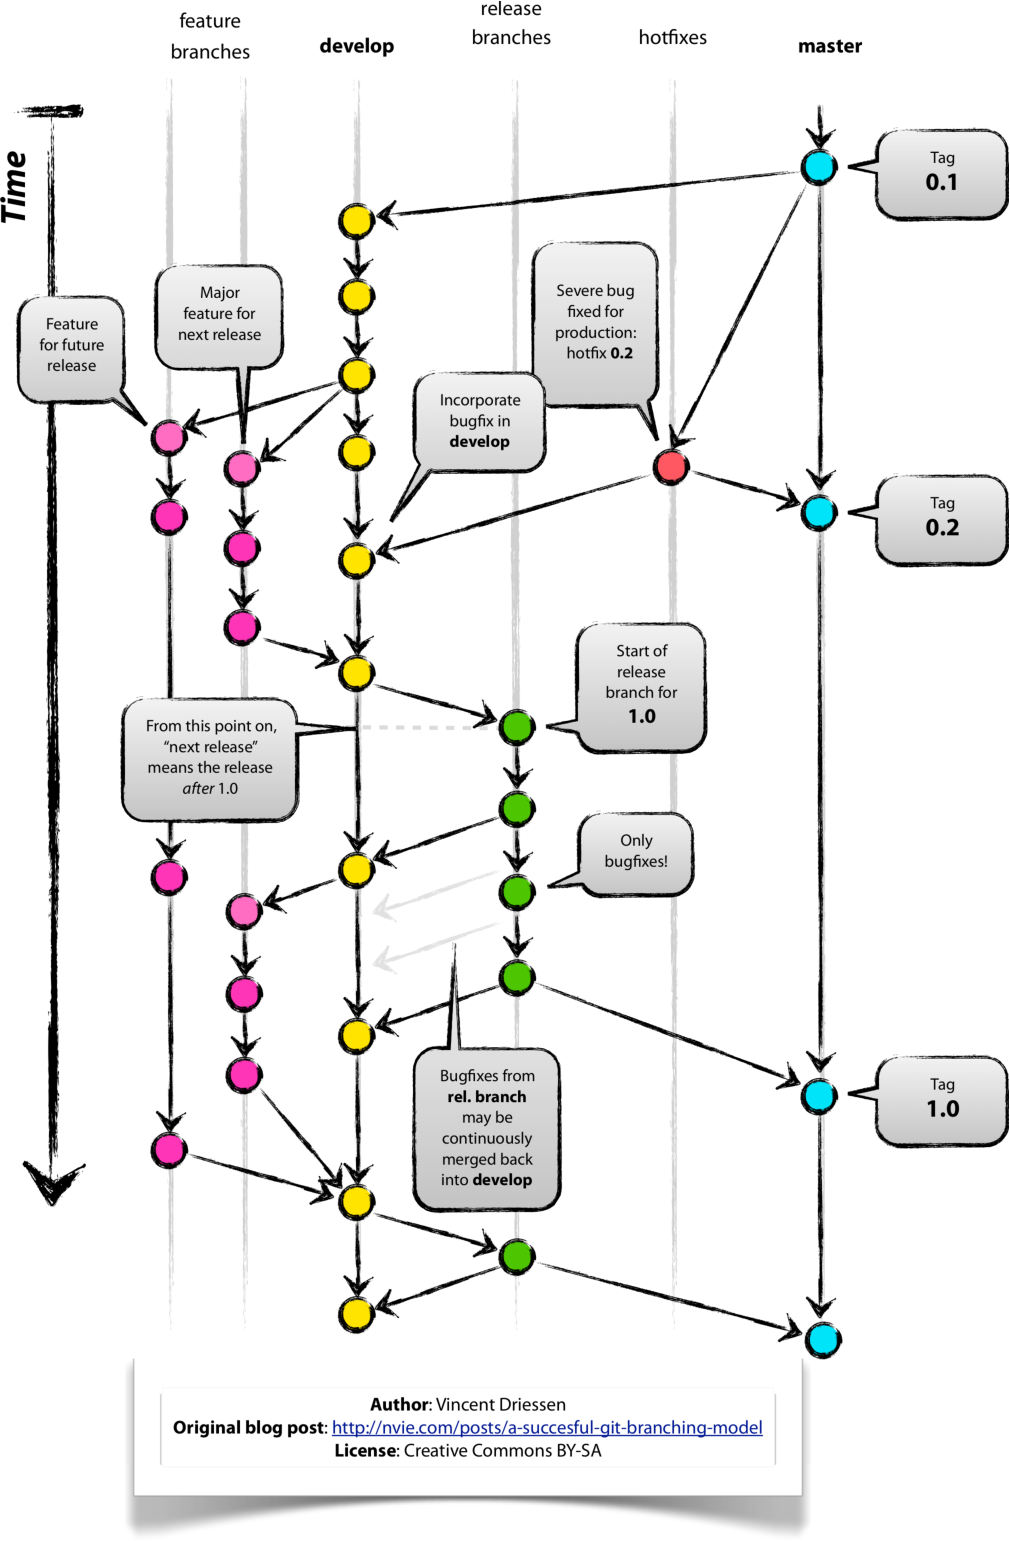
\includegraphics[width=.9\textwidth]{./Figures/Git-branching-model.pdf}
	\caption[Modelo de ramas utilizado en git]{Modelo de ramas utilizado en git\protect\footnotemark.}
	\label{fig:branching}
\end{figure}

\footnotetext{Imagen tomada de \url{https://nvie.com/files/Git-branching-model.pdf}.}

La mecánica de trabajo indica crear una nueva rama por cada característica a implementar.  Cuando la característica se logra, se debe hacer \textit{merge} con la rama \textit{develop} cuidando que no suceda un \textit{fastforward} y se pierdan los \textit{commits} de la rama recién integrada.

Para este trabajo, se crearon ramas para desarrollar cada uno de los subsistemas mencionados en el diagrama en bloques de la figura \ref{fig:diagramaBloquesReducido} e incluidos en el alcance del trabajo, a saber:

\begin{itemize}
	\item \textit{sdcard} para el módulo de almacenamiento.
	\item \textit{onewire} para el módulo de adquisición.
	\item \textit{hmi} para el módulo de interfaz con el usuario.
	\item \textit{control} para el módulo de control.
	\item \textit{ceedling} para el entorno de testing.
\end{itemize}  

\subsection{Paradigma de desarrollo basado en pruebas}
\label{subsec:tdd}

El paradigma de desarrollo basando en pruebas o TDD (por sus siglas en inglés, \textit{Test Driven Development}) \citep{beck2003test} es una práctica de programación que forma parte de las metodologías ágiles.  TDD plantea invertir el orden tradicional de desarrollo en el cual primero de implementa y luego se prueba.  En este sentido, este paradigma propone un proceso de desarrollo que consiste en codificar pruebas, desarrollar y refactorizar de forma iterativa el código.

Si bien no se adoptó el modelo de desarrollo TDD en forma íntegra, sí se incorporaron algunos de sus principios a la metodología de trabajo, en particular los que permiten la producción de un \textit{firmware} modular, altamente reutilizable y preparado para el cambio, es decir escalable, conocidos como principios ``SOLID''\citep{martin2000design}:

\begin{itemize}
	\item Principio de responsabilidad única (\textit{Single responsibility principle}). Cada módulo debe tener una única responsabilidad.
	\item Principio de abierto/cerrado (\textit{Open/closed principle}). Un módulo debe estar abierto para su extensión, pero cerrado para su modificación.
	\item Principio de sustitución de Liskov (\textit{Liskov substitution principle}). Los objetos de un programa deberían ser reemplazables por instancias de sus subtipos sin alterar el correcto funcionamiento del programa.
	\item Principio de segregación de la interfaz (\textit{Interface segregation principle}). Muchas interfaces cliente específicas son mejores que una interfaz de propósito general.
	\item Principio de inversión de la dependencia (\textit{Dependency inversion principle}). Depender de abstracciones, no depender de implementaciones.  Esto significa que un módulo A no debe depender de otro módulo B, sino a través de una abstracción de B.
\end{itemize}

Asimismo, se tomó de TDD la filosofía de pensar primero cómo se va a probar que el código cumple los requerimientos para lograr un mejor entendimiento del sistema y aumentar la calidad del diseño.

En el capítulo \ref{Chapter4} se recopila la documentación de casos de prueba que se usaron como entrada al diseño del \textit{firmware} previo de su implementación.

\subsection{Programación concurrente con Protothreads} 
\label{subsec:protothreads}

Los Protothreads son una abstracción creada por Adam Dunkel para implementar mecanismos de programación concurrente, conocidos como multi-tarea cooperativa, en sistemas embebidos con recursos limitados \citep{Protothreads}. 

Se distribuyen como una biblioteca que puede integrarse al proyecto y posibilitan trabajar con hilos de ejecución sin \textit{stack} o co-rutinas, con mecanismos para bloquear la ejecución de una tarea sin que se produzca un cambio de contexto.  Esto permite un control de flujo secuencial sin máquinas de estado complejas o soporte multi-hilo completo en arquitecturas basadas en eventos \citep{dunkels06protothreads} \citep{dunkels05using}. 

Los protothreads se implementan como un conjunto de macros que el precompilador expande en tiempo de compilación.  

\begin{verbatim}
	struct pt { unsigned short lc; };
	#define PT_THREAD(name_args)  char name_args
	#define PT_BEGIN(pt)          switch(pt->lc) { case 0:
	#define PT_WAIT_UNTIL(pt, c)  pt->lc = __LINE__; \
	                              case __LINE__: \
	                              if(!(c)) return 0
	#define PT_END(pt)            } pt->lc = 0; return 2
	#define PT_INIT(pt)           pt->lc = 0
\end{verbatim}

%\end{lstlisting}
En los algoritmos \ref{lst:proto1} y \ref{lst:proto2} se puede apreciar un ejemplo sencillo que utiliza esta herramienta y el mismo código con las macros expandidas, respectivamente. El \textit{quid} de la implementación es la utlización de una estructura \texttt{switch} y la macro \texttt{\_\_LINE} para insertar el número de línea y permitir la reentrada a una parte del código. En este ejemplo, \texttt{PT\_WAIT\_UNTIL} se encuentra en la línea 12.

\noindent\begin{minipage}{.5\textwidth}
\begin{lstlisting}[caption=Ejemplo de uso,frame=tlrb,basicstyle=\footnotesize,label={lst:proto1}]{Name}
static
PT_THREAD(example(struct pt *pt))
{
  PT_BEGIN(pt);
  
  while(1) {
    PT_WAIT_UNTIL(pt,
      counter == 1000);
    printf("Threshold reached\n");
    counter = 0;
  }
  
  PT_END(pt);
}
\end{lstlisting}
\end{minipage}\hfill
\begin{minipage}{.5\textwidth}
\begin{lstlisting}[caption=Código expandido,frame=tlrb,basicstyle=\footnotesize,label={lst:proto2}]{Name}
static
char example(struct pt *pt)
{
  switch(pt->lc) { case 0:
 
  while(1) {
    pt->lc = 12; case 12:
    if(!(counter == 1000)) return 0;
    printf("Threshold reached\n");
    counter = 0;
  }
 
  } pt->lc = 0; return 2;
}
\end{lstlisting}
\end{minipage}

Se debe tener en cuenta que por la forma en que están implementados, no es posible incluir bloques de control \texttt{switch-cese} dentro de los protothreads.	

En el presente trabajo, se hace uso de protothreads en la codificación del protocolo de comunicación 1-wire que se describe en la subsección \ref{subsec:1-wire}.


\section{Arquitectura multicore}
\label{sec:arquitectura}

El \textit{firmware} está desarrollado sobre la base de dos proyectos vinculados dentro IDE MCUXpresso, uno para cada \textit{core} del microcontrolador. Para el IDE, debe haber un proyecto ``maestro'' que controle la ejecución del código (o al menos la secuencia de \textit{startup}) corriendo en el otro \textit{core}, considerado ``esclavo''.  

El proyecto maestro contiene un link al proyecto esclavo que produce que la imagen binaria del esclavo sea incluida en la imagen  binaria del maestro, cuando el proyecto maestro es compilado \citep{nxp:mcuxpresso}. De esta manera, cuando el proyecto maestro es grabado en la flash del microcontrolador, ambos proyectos son descargados a la memoria del microcontrolador.

El proyecto maestro debe ser el que se ejecuta sobre el procesador Cortex-M4 ya que el procesador Cortex-M0 permanece en estado de \textit{reset} hasta que el otro \textit{core} lo libera de este estado escribiendo un 0 en el bit M0SUB\_RST del registro RESET\_CTRL1, como se indica en el manual del microcontrolador \citep{nxp:lpc4337}.

Cuando se energiza el microcontrolador o se produce un \textit{reset}, el \textit{core} maestro inicia su secuencia de \textit{startup} y es responsable de iniciar, a su vez, la secuencia de \textit{startup} del \textit{core} esclavo.  

En las tablas \ref{tab:memoriaM4} y \ref{tab:memoriaM0} se muestra la asignación de bloques de memoria para los procesadores Cortex-M4 y Cortex-M0, respectivamente.  Puede verse que el código de cada procesador se ubica en un bloque de memoria flash independiente, los bancos A y B de 512 kB cada uno.  

Por otra parte, para evitar cualquier tipo de solapamiento en el uso de la RAM, los proyectos asociados a cada \textit{core} se linkean de forma de utilizar exclusivamente bancos de RAM separados.  En este sentido, el procesador cortex-M4 utiliza el primer bloque de RAM de 32 kB y el procesador cortex-M0 utiliza el segundo bloque de RAM de 40kB.

\begin{table}[ht]
\centering
\caption{Asignación de bloques de memoria para el Cortex-M4}
\begin{tabular}{lllll}
\toprule
\textbf{Tipo de memoria} & \textbf{Nombre} & \textbf{Alias} & \textbf{Ubicación} & \textbf{Tamaño} \\ 
\midrule
Flash                    & MFlashA512      & Flash          & 0x1a000000         & 0x80000         \\
RAM                      & RamLoc32        & RAM            & 0x10000000         & 0x8000          \\ 
\bottomrule
\end{tabular}
\label{tab:memoriaM4}
\end{table}

\begin{table}[ht]
\centering
\caption{Asignación de bloques de memoria para el Cortex-M0}
\begin{tabular}{lllll}
\toprule
\textbf{Tipo de memoria} & \textbf{Nombre} & \textbf{Alias} & \textbf{Ubicación} & \textbf{Tamaño} \\ 
\midrule
Flash                    & MFlashB512      & Flash2          & 0x1b000000         & 0x80000         \\
RAM                      & RamLoc40        & RAM2            & 0x10080000         & 0xa000          \\ 
\bottomrule
\end{tabular}
\label{tab:memoriaM0}
\end{table}

Adicionalmente, se define una zona de memoria compartida, visible por ambos procesadores para el intercambio de información. Los mecanismos de comunicación inter-procesadores (IPC, del inglés \textit{Inter Processor Communication}) se describen en la sección \ref{subsec:IPC}. 

\begin{verbatim}
/* Shared memory used by IPC */
#define SHARED_MEM_IPC   0x10088000	 
\end{verbatim}

\subsection{Inter Processor Communications}
\label{subsec:IPC}

Para comunicar ambos procesadores se utiliza una biblioteca provista por el fabricante del microcontrolador NXP, documentada en la nota de aplicación ``AN1117: Inter Processor Communications for LPC43xx'' \citep{nxp:an1117}. En este documento se explican mecanismos posibles para que los dos procesadores intercambien información basados en interrupciones, en colas de mensajes y en ``casillas de correo''.  Este último método queda excluido de esta memoria por no haber sido utilizado en el desarrollo.

\subsubsection{Interrupciones cruzadas}
\label{subsubsec:interrupcion}

El mecanismo de interrupciones cruzadas es el más simple de los tres métodos provistos.  Permite que un \textit{core} active una interrupción en el otro \textit{core} para enviar notificaciones cuya interpretación depende y es exclusiva de la aplicación.  El diseñador puede definir una función de \textit{callback} que es ejecutada en el contexto de la rutina de servicio de la interrupción.  

Para enviar señales al \textit{core} ``remoto'', el \textit{core} ``local'' utiliza una instrucción dedicada SEV (\textit{send event}) provista por la arquitectura Cortex.

Asimismo, dentro de la rutina de interrupción se habilita un \textit{flag} para indicar que se ha recibido una notificación IPC.  Esta variable \textit{flag} puede ser usada por las aplicaciones corriendo sobre el \textit{core} que recibe la notificación para chequear el estado de las comunicaciones. 

La limpieza del \textit{flag} se hace dentro de una sección crítica donde se deshabilitan temporalmente las interrupciones. En el Cortex-M4 se enmascaran las interrupciones con mayor prioridad y en el Cortex-M0 se deshabilitan directamente, ya que este procesador no dispone del mecanismo de enmascaramiento.

El código para generar las interrupciones cruzadas utiliza dos macros. Primero \_\_DSB() (\textit{Data Syncronization Barrier}) para terminar todas las transacciones de memoria pendientes y luego \_\_SEV() (\textit{Send Event}) para generar el envío de una señal de interrupción al otro procesador como puede verse en el algoritmo \ref{lst:ipc_send_signal}.

\begin{lstlisting}[caption={Función ipc\_send\_signal que permite generar una interrupción en el otro procesador.},label={lst:ipc_send_signal}]
/*
 * Initiate interrupt on other processor
 * Upon calling this function generates and interrupt 
 * on the other core. Ex. if called from M0 core it 
 * generates interrupt on M4 core and vice versa.
 */
static void ipc_send_signal(void)
{
  	__DSB();
  	__SEV();
}
\end{lstlisting}

\subsubsection{Colas de mensajes}
\label{subsubsec:colas}

En el método de colas de mensajes, se deben definir dos áreas de memoria compartida, que se utilizan para almacenar los mensajes que cada procesador envía al otro. Una cola (búfer de comandos del \textit{host}) está dedicado a los comandos enviados del procesador maestro al esclavo, y una cola (búfer de mensajes del \textit{host}) se dedica a los mensajes que el procesador esclavo envía en respuesta al procesador maestro. La figura \ref{fig:IPC} muestra esquemáticamente esta configuración.

\vspace{15px}

\begin{figure}[!htpb]
	\centering
	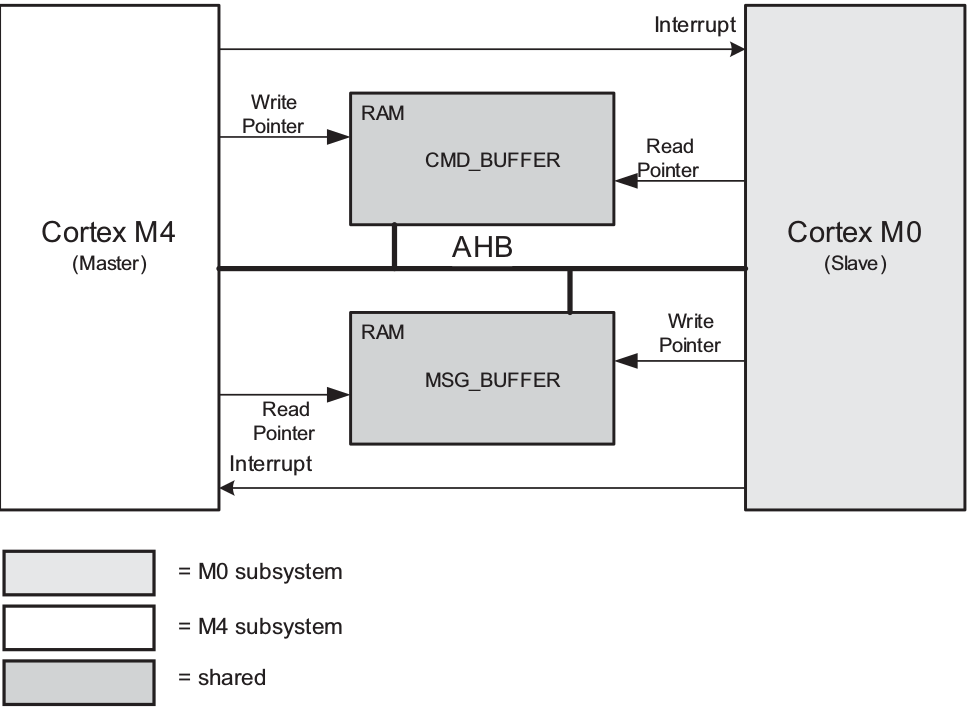
\includegraphics[width=\textwidth]{./Figures/IPC.png}
	\caption[Esquema de comunicación entre procesadores]{Esquema de comunicación entre procesadores basado en colas de mensajes\protect\footnotemark.}
	\label{fig:IPC}
\end{figure}

\vspace{15px}
%\vfill
\footnotetext{Imagen tomada del manual de usuario del microcontrolador LPC4337 \citep{nxp:lpc4337}}

En el esquema propuesto, sólamente el procesador maestro puede escribir en el búfer de comandos y recibe los mensaje del esclavo leyendo el búfer de mensajes.  De manera análoga, únicamente el esclavo puede escribir en el búfer de mensajes y recibe comandos leyendo el búfer de comandos.

Cuando un procesador escribe un nuevo mensaje en una cola, debe notificar al otro procesador de que hay nueva información para procesar. Para tal fin, se utiliza el mecanismo de interrupción descripto en el apartado Interrupciones cruzadas, dentro de la subsección \ref{subsubsec:interrupcion}.

El procesador que recibe el mensaje invoca a un despachador de eventos que busca en un vector de manejadores de eventos el que haya sido registrado para tal fin. En el algoritmo \ref{lst:ipc_dispatcher} se pude apreciar la función provista por la bilbioteca IPC para despachar eventos.

\vspace{10px}

\begin{lstlisting}[caption={Función despachadora de eventos de la biblioteca IPC.},label={lst:ipc_dispatcher}]
/* This task will receive the message from the other 
 * core and will invoke the appropriate callback with
 * the message
 */
static void ipcex_dispatch_task(void *unused)
{
  int ret;
  ipcex_msg_t msg;
  	do {
    	ret = IPC_popMsgTout(&msg, -SYS_OS_ID);
    	if((ret != QUEUE_VALID) || 
                      (msg.id.pid >= IPCEX_MAX_PID)){
      	continue;
    	}
    	if (ipcex_callback_lookup[msg.id.pid]) {
      	ipcex_callback_lookup[msg.id.pid](&msg);
    	}
  	} while (SYS_OS_ID);
}
\end{lstlisting}
\vspace{5px}
SYS\_OS\_ID es una macro que se utiliza para identificar el tipo de Sistema Operativo incluido en la aplicación.  En el caso particular de este trabajo, SYS\_OS\_ID es igual a 0 y esto significa que no hay Sistema Operativo.  Se debe notar que SYS\_OS\_ID = 0 implica que el despachador de eventos se ejecuta una única vez por mensaje recibido.

La función despachadora de eventos descripta en el algoritmo \ref{lst:ipc_dispatcher} fue modificada para adaptarla a las necesitadas del proyecto.  En la sección \ref{sec:control} se documenta cómo se implementó esta función dentro del módulo de control de la estación de monitoreo de ruido acústico.

Para el intercambio de mensajes en el sistema, se define un nuevo tipo de dato \texttt{ipcex\_msg\_t}.  Se trata de una estructura que contiene información que identifica al CPU y al proceso destinararios del mensaje, definidos dentro de otra estructura anidada, junto con dos campos para datos como se observa en el algoritmo \ref{lst:ipcex_msg_t}. 

\begin{lstlisting}[caption={Definición de un nuevo tipo de dato ipcex\_msg\_t para intercambio de mensajes.},label={lst:ipcex_msg_t}]
typedef struct __ipcex_msg {
  struct {
    uint16_t cpu;
    uint16_t pid;
  } id;

  uint32_t data0;
  uint32_t data1;
} ipcex_msg_t;
\end{lstlisting}

El tipo de datos \texttt{ipcex\_msg\_t}, tal como viene definido en la biblioteca IPC fue modificado como se documenta en la sección \ref{sec:control}.
